\subsection*{Jejdové} % (fold)
\label{sub:jejdové}

\begin{multicols}{2}
	


Mini manévry\\
První den tábora po obědě nám stavebkářům řekli, že si máme zabalit na přespání. Poté jsme se vydali do Ostrovce na nádraží, kde jsme se setkali s ostatními, kteří přijeli vlakem. Poté přišli mnich a sedlák a ti nás rozdělili do dvou skupin a rozdali nám kusy prádelky, na kterou jsme si pověsili vše potřebné vše potřebné na přespání, takže např. spacák, karimatku, pití a kartáček na zuby. Prádelku jsme si pověsili buď kolem pasu, nebo na rameno. Poté mnich a sedlák každé skupině dali popis cesty a my se vydali vstříc cestě. Cesta ubíhala dobře, až jsme se dostali do bodu zlomu. Rozdělili jsme se na dvě skupiny. Jedna chtěla jít rovně a druhá doleva. Nakonec vyhrála skupina vlevo. Tak jsme se po půl hodině improvizování dostali do vesnice… Ostrovec. Tam jsme zavolali na číslo na našem papíře a dovolali jsme se překvapivě do tábora. Když jsme jim oznámili, že jsme se dostali opět do Ostrovce, byli velice překvapeni. Poradili nám a doplnili jsme zásoby vody a opět se vydali na cestu. Když jsme se opět dostali do onoho bodu, tentokrát jsme se vydali rovně a po chvíli jsme se chytili popisu. Podle něj jsme pokračovali asi do tři čtvrtě cesty, kde jsme najednou potkali druhou skupinu, která se u silnice a nevěděla kam dál. Poté jsme podle popisu pokračovali až do obce Zvíkov. V obci jsme se měli vydat podél tří hostinců a dvou tee-pee. Po chvíli jsme narazili na paní a po dlouhém rozhovoru s ní jsme zjistili, kde bydlí pán, který staví tee-pee. Ten nám řekl, že právě dvě tee-pee stojí u dětského domova a ukázal nám cestu. Po chvíli jsme se dostali k rozcestí dvou cest a opět jsme nevěděli kam dál. Opět jsme se rozdělili na dvě skupiny a jedna zůstala na rozcestí a druhá, ve které jsem byla i já, se vydala hledat dětský domov. Po pár minutách jsme došli k policejní stanici, před kterou stáli dva policisté, a já se bez rozmýšlení jednoho z nich zeptala, kde je tu dětský domov a oni nám řekli kudy. A tak jsme se konečně dostali k dětskému domovu a já se vydala pro druhou skupinu, ale jinou cestou, která měla být rychlejší. Po chvíli jsem se dostala k rozcestí, kde měla druhá skupina čekat, ale nebyla tam a tak jsem se vrátila k dětskému domovu a naštěstí druhá skupina za chvilku dorazila. Společně jsme se vydali dál k hradu Zvíkov. Tam nás po chvilce hledání našli mnich se sedlákem a společně jsme si dali večeři neboli chleby s májkou. Při večeři nám vyprávěli, že lidé co zde žijí, jsou zapřisáhlí monarchisté a jelikož jsme demokrati, tak jsme museli odtamtud co nejrychleji odejít a tak jsme hned po večeři vyrazili do lesa kousek od hradu a tam se utábořili. Ráno nás vzbudil voják, který přišel sebrat mnicha jako vzbouřence proti režimu. Když z nás opadl šok, přišli muž a žena, kteří se představili jako Namežan a Žužuman Delaff. Ti nás pozvali na svoji loď, na které budeme podnikat cesty do různých koutů naší země a přesvědčovat lidi, aby podporovali demokracii. A tak jsme se se sedlákem vydali na, teď už i naši, loď neboli do tábora. A toto byl stručný zápis událostí prvních dvou dnů našeho tábora.

\podpis{Mrkev}



Letos jsem si hodně užila tábor. První den jsme vyrazili na "minimanévry" . Byli jsme na hradě Zvíkově aby jsme zachránili demokracii před monarchií. Jako piráti jsme se snažili aby monarchisté pochopili proč chceme demokracii. To se nám na konci tábora podařilo, pomocí elixíru pochopení.
První trojdenka byla s kibitzem. Na trojdence jsme velice zapojili svou fantazii.
Byli jsme tam i s Borúwkama. Kája a Zubejda přijeli pozdě, ale přivezli dort,(protože Kája měla narozeniny).Trojdenku i dort jsme si všichni užili.
Na další trojdence jsme začali celoroční téma u kterého nás měla provádět kniha: Kronika rodu Spiderwicků. Za celou trojdenku jsme přečetli dva díly. Hlavní pointou trojdenky bylo zahnání zlého polykače na dvacet let do podsvětí. Zahánění polykače jsme absolvovali my osobně a aby polykač neřádil ve městě moc dlouho i za dalších třicet let , kdy už bude moct znovu opustit podsvětí tak jsme jedné místní paní dali instrukce aby i ona (nebo její potomci) mohla vykonat rituál. Až když jsme předali poselství tak jsme se s klidem mohli vrátit do svých domovů.

\podpis{KECKA}




Půlnoční esej\\
Tento tábor jsem slibovala na skauta.
Na přípravách jsme se dozvěděli že musíme napsat esej na to proč sechceme stát skautem.
A čas plinul za pár dnů byl čas odevzdat esej.
Já Zubejda a Penny jsme to měli napsané ale mě a Penny se esej stratila. Už byl večer a byli přípravy a popravy.
Tuto přípravu jsme měli už odevzdávat esej až na to že já a Penny jsme jí pořád neměli. Potom na přípravě nám vedoucí řekly že to tolik nevadí a že to ráno musíme odevzdat.
Po večeři zjistila že mám hlídku a po mě hned Lochneska a rozhodla jsme se že poprosím Lochnesku jestli bych s ní nemohla zůstat na hlídku abych mohla napsat esej.
Když jsem přišla do týpka tak mě poprosila Penny jestli bych ji nevzbudila až budu budit Lochnesku tak jsem souhlasila. Ke konci mé hlídky jsem šla vzbudit Penny i Lochnenesku. Teprve ke konci Lochnesčiný hlídky jsen dopsala konečně esej. Lochneska prosila jestli bych tam sní ještě nezůstala ale už jsem byla moc unavená. tak jsem šla spát.


\podpis{asi Zpátečka}


Zážitku z táborů je velmi hodně bylo těžké se rozhodnout o kterém napíšu . Ale vybrala jsem si noční hru z tábora ( téma: piráti ). Měli jsme jenom přejít křižovatku a zahnout doprava. Nebylo to ale tak lehký protože jsme šli po jednom a museli jsme se plazit. Nebo alspoň být jenom zkrčený. U ty křižovatky však byli něací opilí piráti ( nebo nevim kdo to byl). Takže jste museli být potichu aby vás neslyšeli a nechytli vás. Když jste odbočili tak jste pak šli chvíli po pěšince než jste na někoho nenarazili.

\podpis{Zubejda}

\columnbreak

Příspěvek do knihy Keya
Tento rok jsem si vážně užila! Ráda bych řekla něco o táboře. Když jsme přijeli do vesnice Dolní Ostrovec, nešli jsme rovnou do tábora, ale byly tzv. minimanévry. Naše skupinka to nějak popletla a skončili jsme zpátky v Dolním Ostrovci:) Nakonec jsme přespali poblíž hradu Zvíkov a ráno jsme šli do tábora. Ten den bylo snad naposledy slunce (teda kromě konce tábora). Stavění a dodělávání tee-pee se protáhlo na déle než bychom čekali. Na tomto táboře se nikdo neobešel bez štípanců od vos a komárů. Ale i přes otravný hmyz jsme na táboře s tématem Piráti opravdu užili spoustu zábavy a mě překvapilo že Vařící etapka byla téměř na začátku tábora. Poté byl čas na Skautské přípravy a popravy. Chtěla jsem na konci tábora skládat Skautský slib a psala jsem esej na téma proč chci být Skautem. Jenomže den před termínem odevzdání jsem ji ztratila a musela jsem ho psát na hlídce! Ne na mojí, ale na Lochnessčinu. Potom byly manévry. Byly vážně super včetně toho, že jsme nemuseli nikam hnát. Po návštěváku se na oblohu opět dostalo slunce a bylo teplo. Ale vyskytl se další problém. Jaksi nám nevsakovala vsakovačka, tak jsme ji s Jejdama vylévaly a našli jsme mrtvou myš! Udělaly jsme jí patřičný pohřeb a ozdobili jí hrob. Následující pokladovka se mi moc líbila. Potom přišel čas na 3. táborák a slibování, stala jsem se Skautkou a všichni jsme spali u táboráku. Moc jsem si to užila a děkuji všem vedoucím za skvělý tábor.

\podpis{Penny}


\end{multicols}

\begin{center}

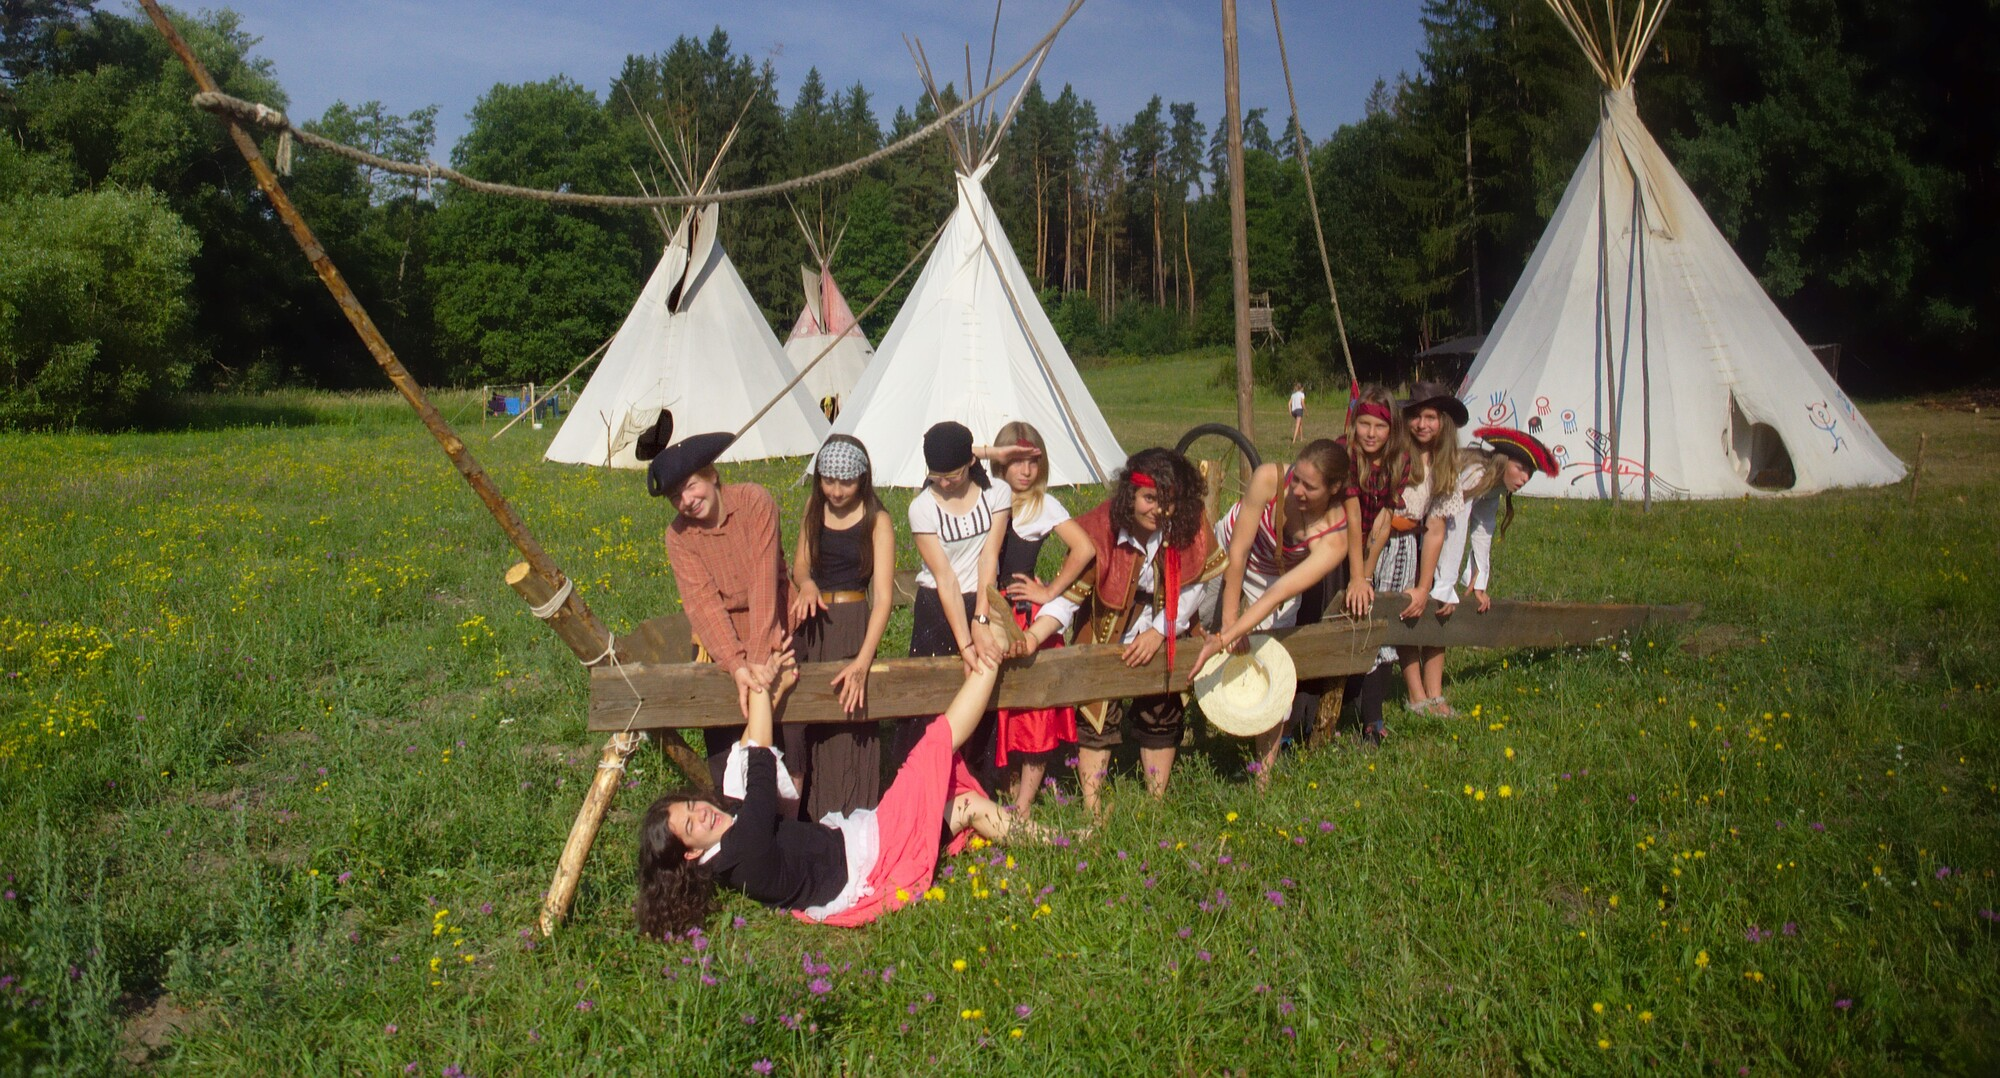
\includegraphics[width=10cm]{img/druziny/jejdove.jpg}

\end{center}


% subsection jejdové (end)